\documentclass{article}
\usepackage[margin=1in]{geometry}
\usepackage{amsmath}
\usepackage{graphicx}

\begin{document}

%Command to change name of table of contents
\renewcommand*\contentsname{Table of Contents}

%Command to start sections on new pages
\newcommand{\sectionbreak}{\clearpage}

\title{\textbf{Performance and Design Calculations}}
\author{Abigail Gries}
\maketitle

This document shows how to calculate important design and performance characteristics of a UAS. 

\newpage

\tableofcontents

\newpage

\section{Variable Definitions}

\begin{itemize}
\item \textit{AR} - The aspect ratio \\
\item \textit{e} - The Oswald Efficiency factor\\
\item $\bar{c}$ - The mean chord length of a wing\\
\item \textit{K} = Wave drag due to lift \\
\item \textit{a} = Slope of $C_L vs \alpha$ \\
\item $C_L$ = Coefficient of lift for a given angle of attack \\
\item $C_{Di}$ = Coefficient of induced drag\\
\item ${C_{D,0}}$ = Coefficient of zero-lift drag\\
\item $C_{fe}$ = Skin friction coefficient\\
\item $S_{wet}$ = Total wetted surface of UAV\\
\item $E_M$ = Maximum aerodynamic efficiency \\
\item \textit{Re} = The Reynolds number\\
\item \textit{Rt} = Battery hour rating\\
\item \textit{n} = Battery discharge parameter\\
\item \textit{V} = Battery voltage\\
\item \textit{C} = Battery capacity\\
\end{itemize}

\newpage

\section{Wing Design}

When designing a wing, the typical first step is to determine the required wingspan, wing planform area, and main airfoil. Additionally, based on the intended flight goals, a taper ratio and sweep angle of the wing also should be chosen. From these preliminary values, the performance of the wing can be calculated. The wing parameters are arguably some of the most influential characteristics on the overall performance of the UAV. \\

\noindent The OpenUAS team has chosen the following preliminary wing characteristics based on the requirements and the intended flight goals. The airfoil selected is NACA 4512 (see Fig. 1 below or Airfoil Documentation). \\

\begin{figure}[ht]
\begin{center}
	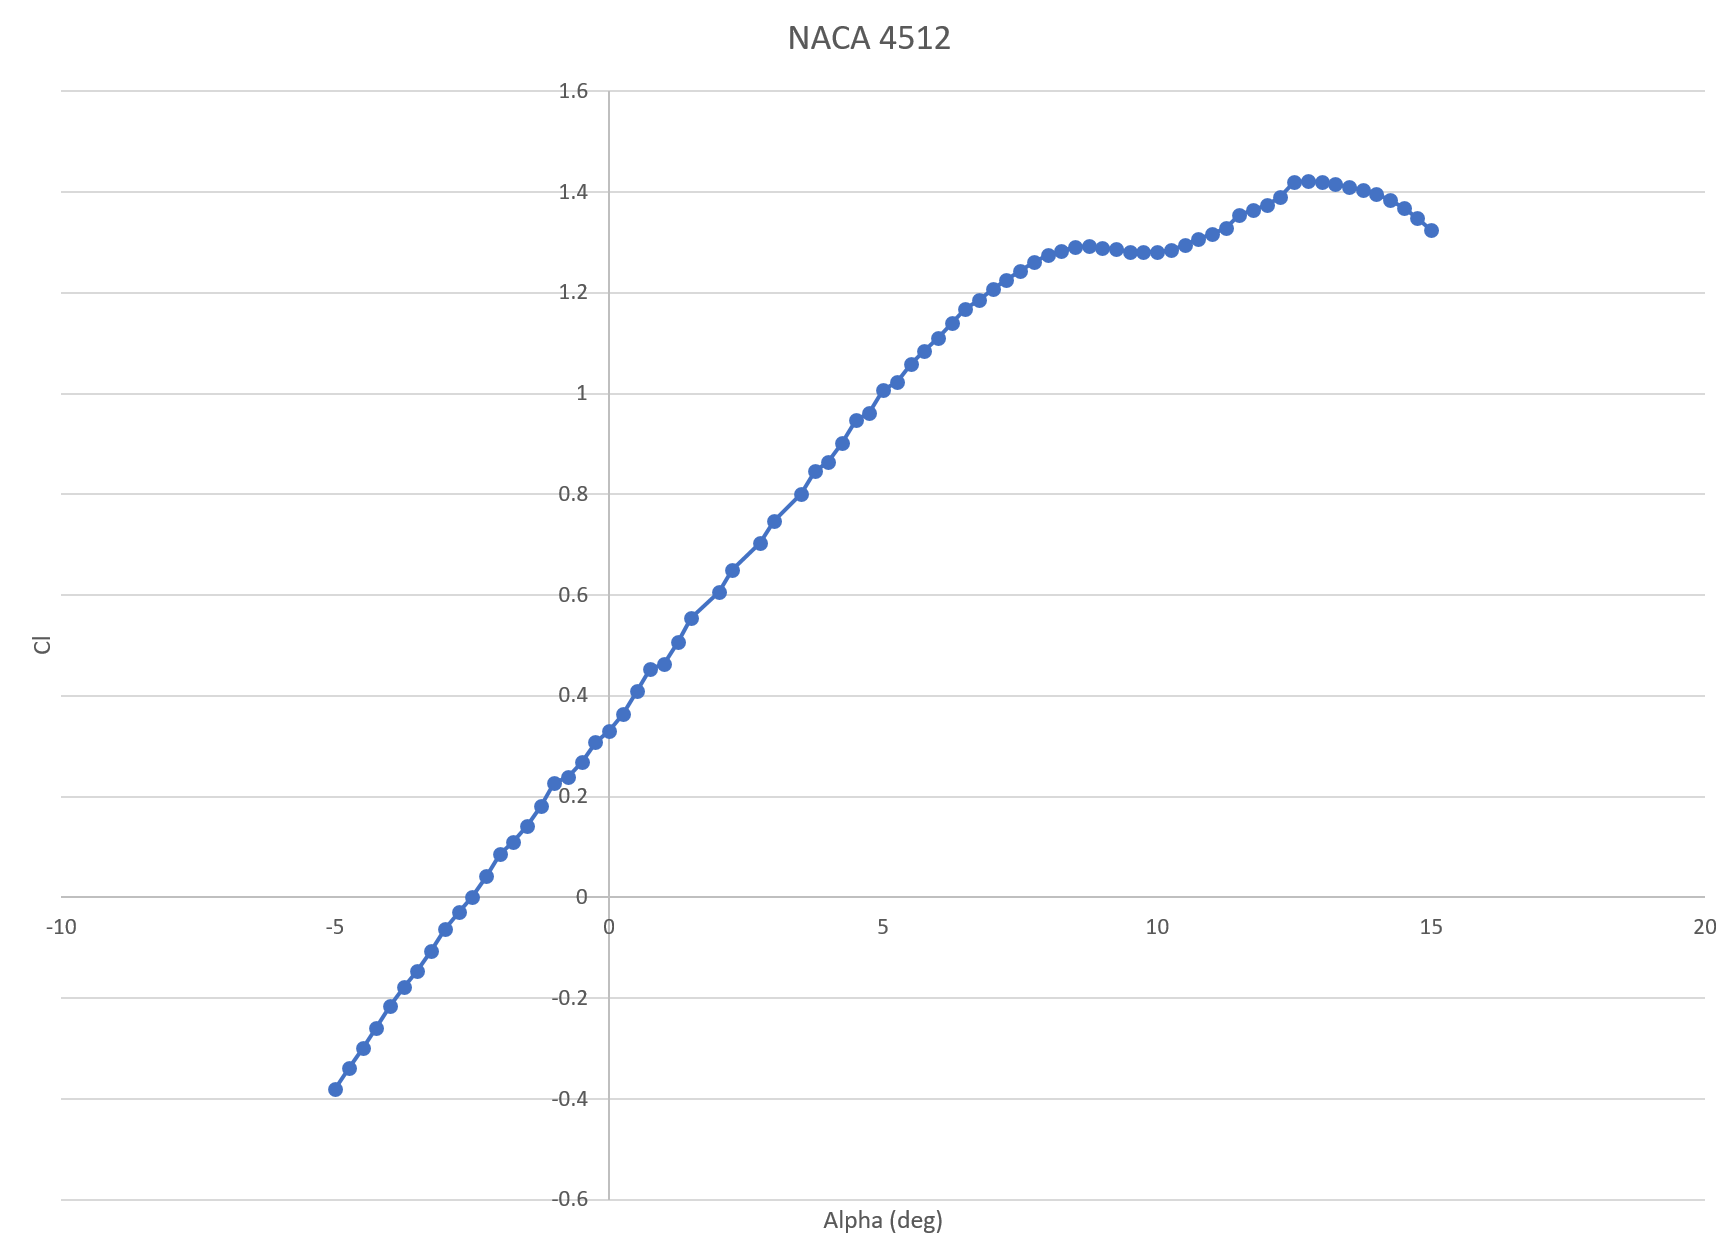
\includegraphics[scale=0.4]{NACA4512clvsalpha.png}
	\caption{NACA 4512 $Cl$ vs $\alpha$}
	\label{Figure 1:}

\end{center}
\end{figure}


\begin{center}
\begin{tabular}[pos]{| c | c | c | c | }
\hline
\textbf{Variable} & \textbf{Description} & \textbf{Value} & \textbf{Units} \\ \hline
\textit{b} & Wingspan & 5 & $ft$ \\ \hline
\textit{S} & Wing Area & 2 & $ft^2$ \\ \hline
$\tau$ & Taper Ratio & 0 & \\ \hline
$\Lambda$ & Sweep Angle & 0 & \textit{degrees} \\ \hline
\textit{$a_0$} & Slope of $C_l$ vs $\alpha$ & 0.134 & \\ \hline
$\alpha_{L=0}$ & Zero Lift Angle of Attack & -2.3 & $degrees$ \\ \hline
\end{tabular} \\~\\
\end{center}

\newpage
\section{Aerodynamics}

Equation 1 demonstrates how to calculate the aspect ratio of a wing. As the aspect ratio of a wing increases, the aerodynamic efficiency of a wing increases as well [1]. The OpenUAS will have a high aspect ratio because the design is almost glider-like. \\
\begin{equation}
AR = \frac{b^2}{S}
\end{equation}
As the true OpenUAS wing is 3D and not an ideal, a correction factor must be applied to certain wing calculations. This correction factor is the Oswald Efficiency factor shown in equation 2 below. \\
\begin{equation}
e =1.78(1-0.45AR^{0.68}) - 0.64
\end{equation}
Equation 3 demonstrates how to calculate the (standard) mean chord length of the wing. 
\begin{equation}
\bar{c} = \frac{S}{b}
\end{equation}
The equation below shows how to calculate $K$, the wave drag due to lift. This value is very useful in estimating important characteristics of the aircraft, such as induced drag, maximum aerodynamic efficiency, and lift of a wing. 
\begin{equation}
K = \frac{1}{\pi eAR}
\end{equation}
Figure 1 above shows the $Cl$ vs $\alpha$ plot for the main airfoil. The slope of the linear line on this plot is $a_0$ and is used to described the selected airfoil. The slope for the wing, $a$ is calculated in equation below. $a_0$ cannot be used in the place of $a$ because the wing is 3D and features of the wing affect the coefficient of the lift produced, thus changing the slope.\\
\begin{equation}
a = \frac{a_0cos(\lambda)}{1+Ka_0cos(\lambda)}
\end{equation}
Using the $a$ value calculated above, the coefficient of lift calculated at any angle of attack can be found with equation 6. \\
\begin{equation}
C_L = a(\alpha - \alpha_{L=0})
\end{equation}
The coefficient of induced drag, or drag due to lift, is estimated using the $K$ and $C_L$ values obtained above. \\
\begin{equation}
C_{Di} = KC_L^2
\end{equation}
The coefficient of zero lift drag is the drag when the lift of an aircraft is equal to zero. This is based on the shape of the aircraft.
\begin{equation}
{C_{D,0}} = C_{fe}\frac{S_{wet}}{S}
\end{equation}
The maximum aerodynamic efficiency describes the best case scenerio lift to drag ratio of an aircraft.
\begin{equation}
E_M = \frac{1}{2\sqrt{KC_{D,0}}}
\end{equation}
\begin{equation}
Re = \frac{\rho v\bar{c}}{\mu}
\end{equation}


\newpage
\section{Take-Off}

\newpage
\section{Climb}

\newpage
\section{Cruise}

\newpage
\section{Landing} 

\newpage
\section{References}

\end{document}
